\chapter{Background}
\label{ch:background}

\section{Chapter Overview}
In this chapter, I introduce two theories central to much of my discourse work: Rhetorical Structure Theory, and speech acts with their underlying communicative intents.

\begin{figure}
    \centering
    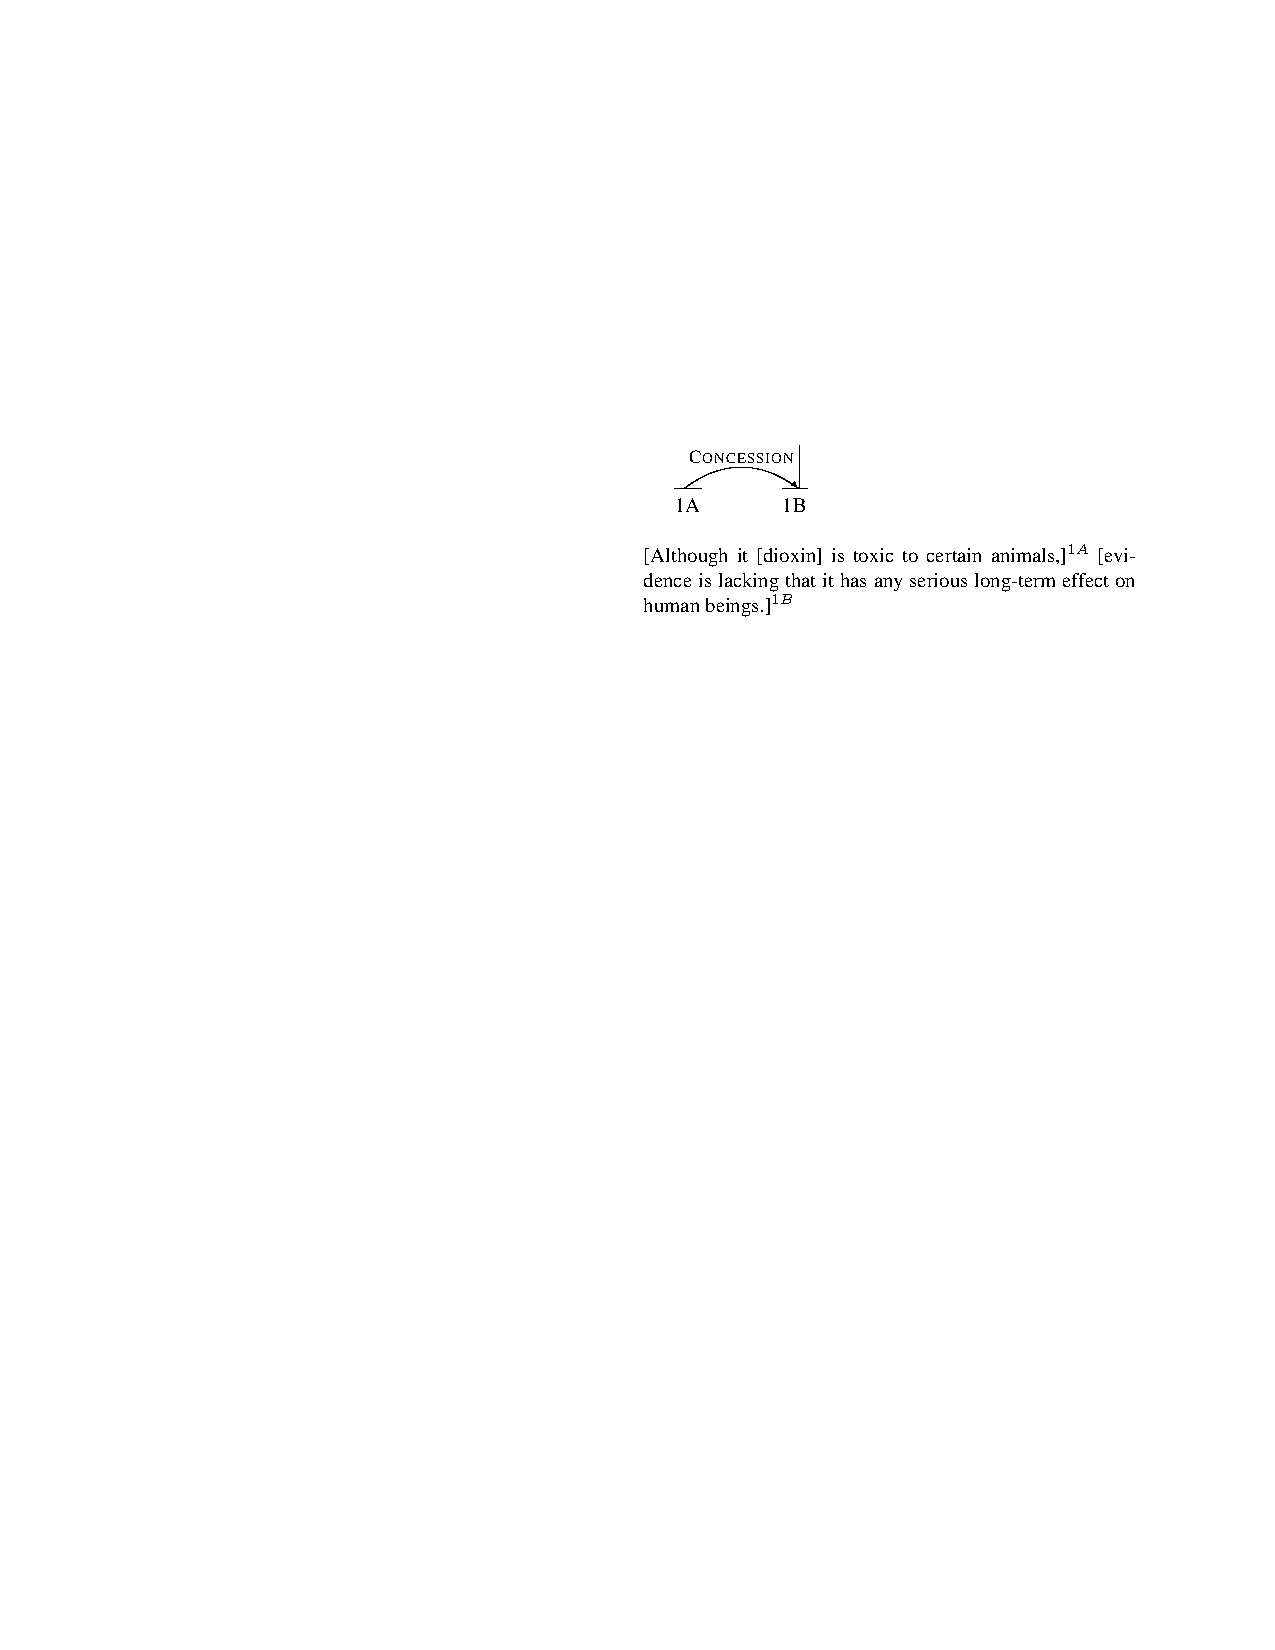
\includegraphics[scale=0.8]{plots/bkgrnd_rst_concession.pdf}
    \caption{Excerpt of RST discourse tree where the nucleus (1B) is the more central part of the \textsc{Concession} relation.}
    \label{fig:bkgrnd_rst_concession}
\end{figure}

% \dirrel{Concession}
% {\rstsegment{\refr{txt1}}}{}
% {\rstsegment{\refr{txt2}}}{}

% \begin{rhetoricaltext}
%   \unit[txt1]{{Although it [dioxin] is toxic to certain animals,}}
%   \unit[txt2]{{evidence is lacking that it has any serious long-term effect on human beings.}}
% \end{rhetoricaltext}

\section{Rhetorical Structure Theory: In theory and in practice}
I present Rhetorical Structure Theory (RST) as it was first theorized and how it evolved as it was operationalized to function within a computational model.  RST is introduced in \citet{Mann:1987} and describes how a text is organized to be coherent and comprehensible, critically through the use of hierarchical relationships that form a tree. Originally developed for natural language generation, RST is meant to capture the intent of the writer and the writer's beliefs of the reader. \citeauthor{Mann:1988} assume the RST analyst has knowledge of the context in which a text was written and of the writer's cultural context in order to make these ``plausibility judgments.'' A relation covers two contiguous spans of text where one span is usually the more central or salient one, termed the nucleus, and the other is the satellite (though multi-nuclear relations also exists where all spans are equally important). The authors present a list of relations defined in terms of the desired effect on the reader from the writer's perspective. In Figure \ref{fig:bkgrnd_rst_concession}, the \textsc{Concession} relation signals the writer's desired effect for the reader to have a positive regard for the nucleus, i.e., dioxin. However, the authors also caution their list of relations is not complete or definitive and should change depending on the focus or genre. Furthermore, arriving at multiple RST analyses of the same text is ``normal'', sometimes arising because there are multiple, simultaneous (i.e., compatible) analyses, but also because of differences between the inherently subjective plausibility judgments of different RST analysts \cite{Mann:1992}.  

Early work that sought to operationalize RST retained the notion of multiple possible discourse trees \cite{Marcu:1996}. With the creation of the RST Discourse TreeBank \cite{Carlson:2001}, the nuances of multiple trees and flexible relation taxonomies were expectedly set aside in order to pave the way for an automated discourse parser that predicts a single tree labelled with a fixed set of relations. Several parsers were proposed and evaluated on their ability to match the structure, nuclearity and relations of the `gold' RST trees \cite{Feng:2014,Ji:2014}. Importantly, a large amount of work shows the discourse information encoded in these trees is useful for several NLP tasks ranging from sentiment analysis \cite{Ji:2017} to summarization \cite{Durrett:2016,Xu:2020}, and in my own work for authorship attribution \newcite{Ferracane:2017} discussed in Chapters \ref{ch:longertexts1} and \ref{ch:longertexts2}. 

However, making effective use of RST trees requires additional abstractions (such as embedding discourse within an entity-centric framework for authorship attribution) or picking only certain parts of the tree (such as focusing on nuclearity for summarization). In an effort to revisit the more flexible view of RST tree that shift with genres or tasks, I explore unsupervised discourse parsing in Chapter \ref{ch:latent} but instead find negative results.  

At the same time, considerable work recognizes ambiguities do arise when creating RST trees. 
\newcite{Das:2017} finds ambiguities are most frequent in the step of labeling the tree, and more so for higher-level nodes that encompass larger spans of text. Even expert annotators labeling ostensibly less subjective texts (news articles)  have differing interpretations. I also find disagreements when manually annotating discourse trees as discussed in Chapter \ref{ch:annotation}, in part due to differences in the annotators' plausibility judgments. This result inspired a focus on the \emph{subjectivity} in discourse, the topic of Chapter \ref{ch:subjective}.

\section{Speech acts and intents}

Speech act theory is first developed in \newcite{Austin:1962} with a focus on performative actions, i.e., how we can do things with words. These acts can be categorized into three kinds: locutionary (the act of speaking), illocutionary (the act done in speaking), and perlocutionary (the effect or consequence of speaking). \newcite{Searle:1969} further defines illocutionary effects (in contrast with perlocutionary effects) as consequences of successful acts that rely on the listener's conventional knowledge. In this theory, however, the listener plays a passive role. \newcite{Bach:1979} instead develop an \emph{intention-centered} theory of speech acts drawing on Grice's conversational implicatures \cite{Grice:1967} to argue that listeners make certain inferences about the intent of the speaker based on their mutual contextual beliefs.  \newcite{VanDijk:1977} similarly argues for speech acts to be described from the perspective of the listener (not just the speaker). \newcite{Cohen:1979} further develops the intentions that underlie speech acts by treating them as plans that affect the beliefs of the speakers and listeners. \newcite{Traum:1992} extend speech acts to dialogue settings, where a \emph{conversation act} can span an entire turn in the conversation (and not be restricted to a single utterance). In my work on subjective discourse in Chapter \ref{ch:subjective}, I elicit judgments on conversation acts and their intents.

\section{Chapter Summary}

In this chapter, I discussed the evolution of RST from theory to practice and how it is beneficial to NLP tasks, but I also take a critical look at some current issues. I next discuss speech act theory and its development to include intents of both the speaker and listener and its extension to conversations.